	\chapter{Deep Learning Prework}
	\section{Artificial Neural Network Regression}

Forward propagation: Going from input (features/data) to output (prediction).

	\subsection{Regression}
 	\begin{figure}[h]
		\centering
		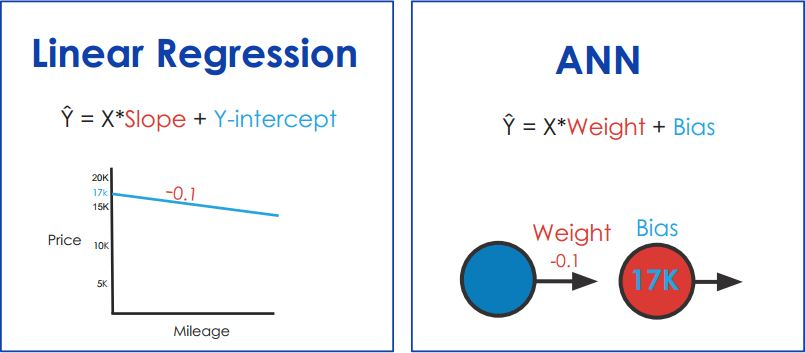
\includegraphics[height=2.0in]{artificialneuralnetworksversuslinearregression}
		\caption{.}
		\label{fig:artificialneuralnetworksversuslinearregression}
	\end{figure}


 	\begin{figure}[h]
		\centering
		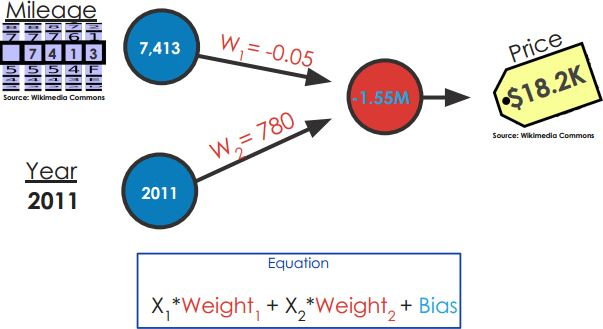
\includegraphics[height=2.0in]{artificialneuralnetworksregressionintro}
		\caption{.}
		\label{fig:artificialneuralnetworksregressionintro}
	\end{figure}

	\subsection{Classification}
With a multi-class classification problem, use the Softmax function to force the probabilities for all classes to sum to one.

 	\begin{figure}[h]
		\centering
		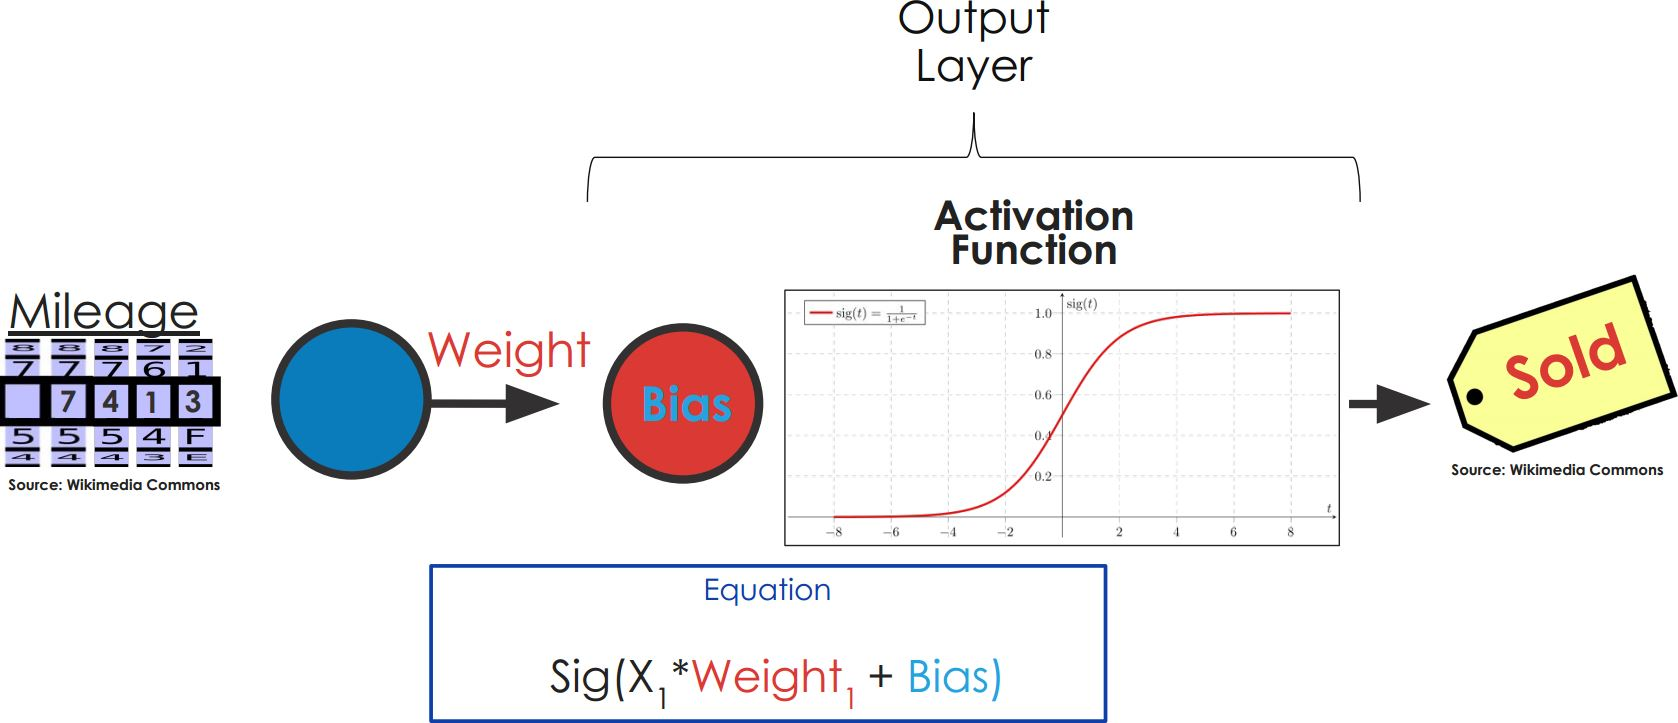
\includegraphics[height=1.8in]{artificialneuralnetworksclassification1}
		\caption{.}
		\label{fig:artificialneuralnetworksclassification1}
	\end{figure}

 	\begin{figure}[h]
		\centering
		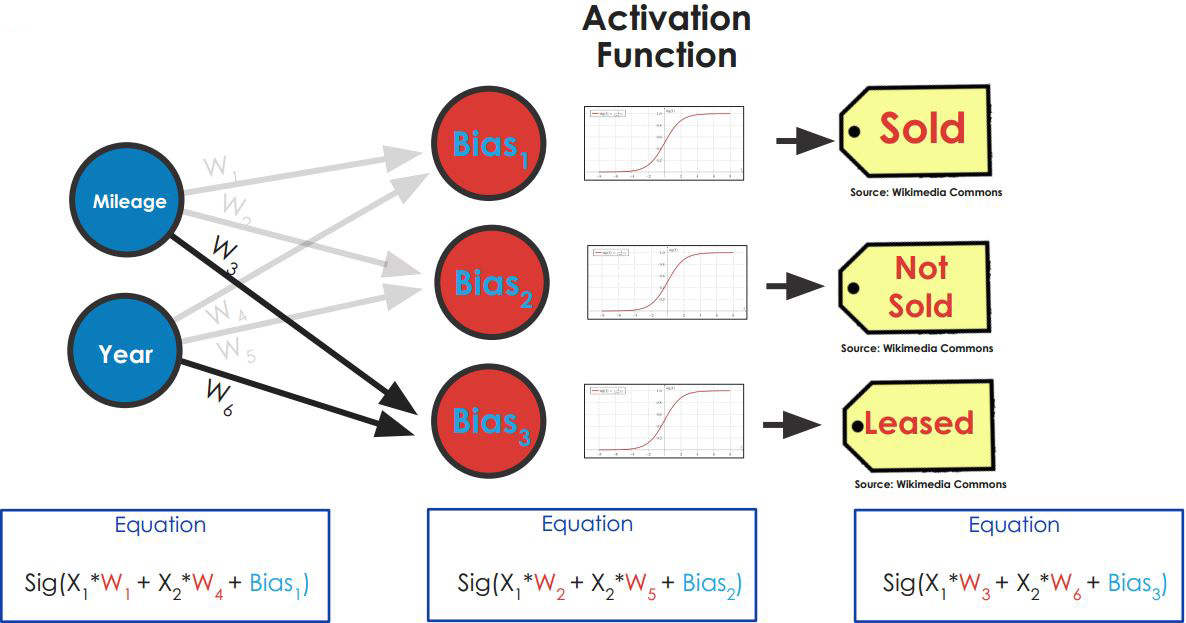
\includegraphics[height=2.3in]{artificialneuralnetworksclassification2}
		\caption{.}
		\label{fig:artificialneuralnetworksclassification2}
	\end{figure}

	\subsection{Tensors}

 	\begin{figure}[tbh]
		\centering
		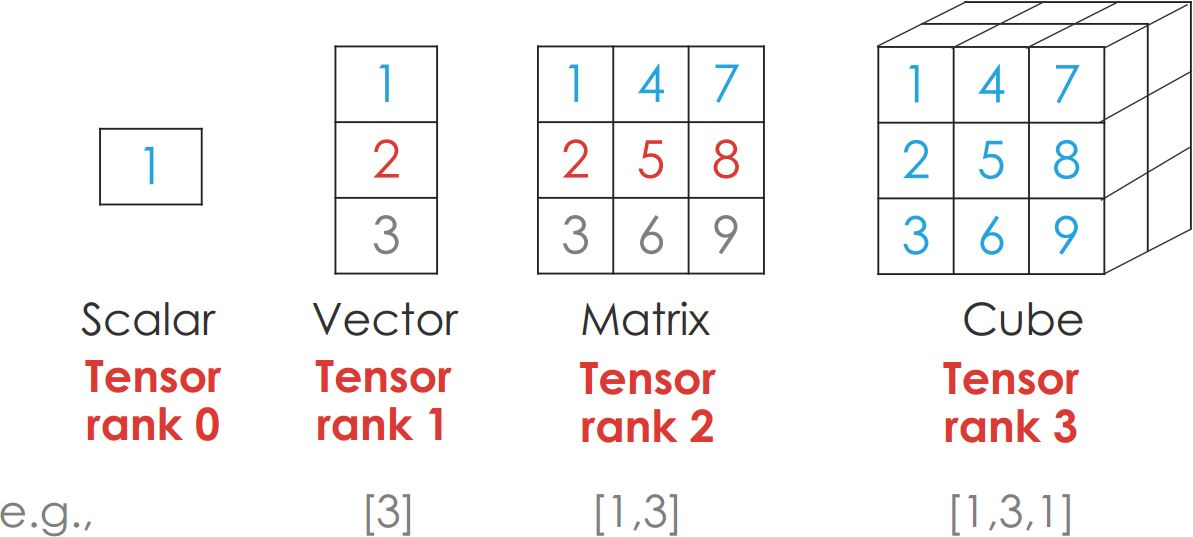
\includegraphics[height=1.5in]{tensors1}
		\caption{.}
		\label{fig:tensors1}
	\end{figure}
 	\begin{figure}[tbh]
		\centering
		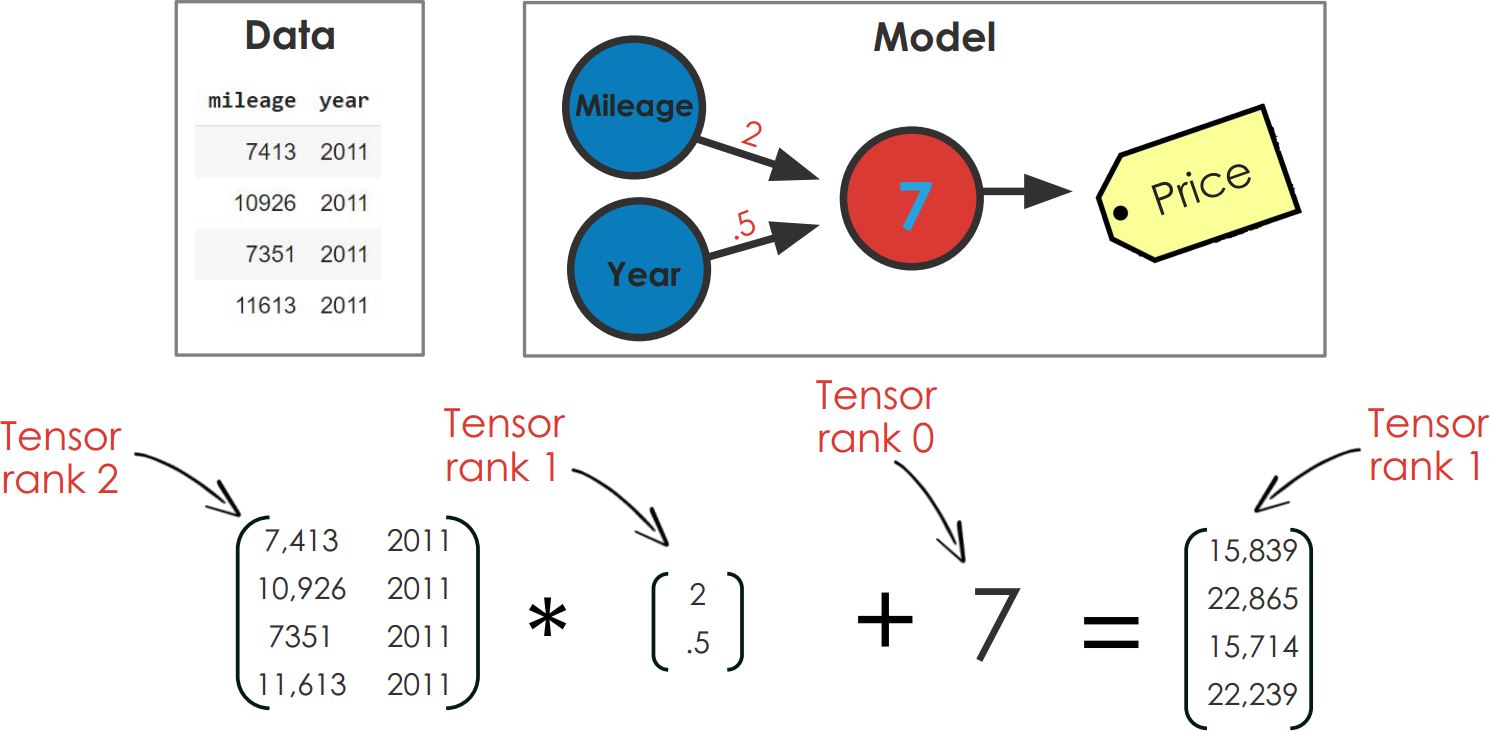
\includegraphics[height=2.0in]{tensors2}
		\caption{.}
		\label{fig:tensors2}
	\end{figure}

	\subsection{Deep Learning}

The perceptron the first attempt at artificial neural network.  It was hardware based.  It took images and interpreted them.  For example, determining which letter it was looking at(\figurename~\ref{fig:deeplearning1}).
 	\begin{figure}[h]
		\centering
		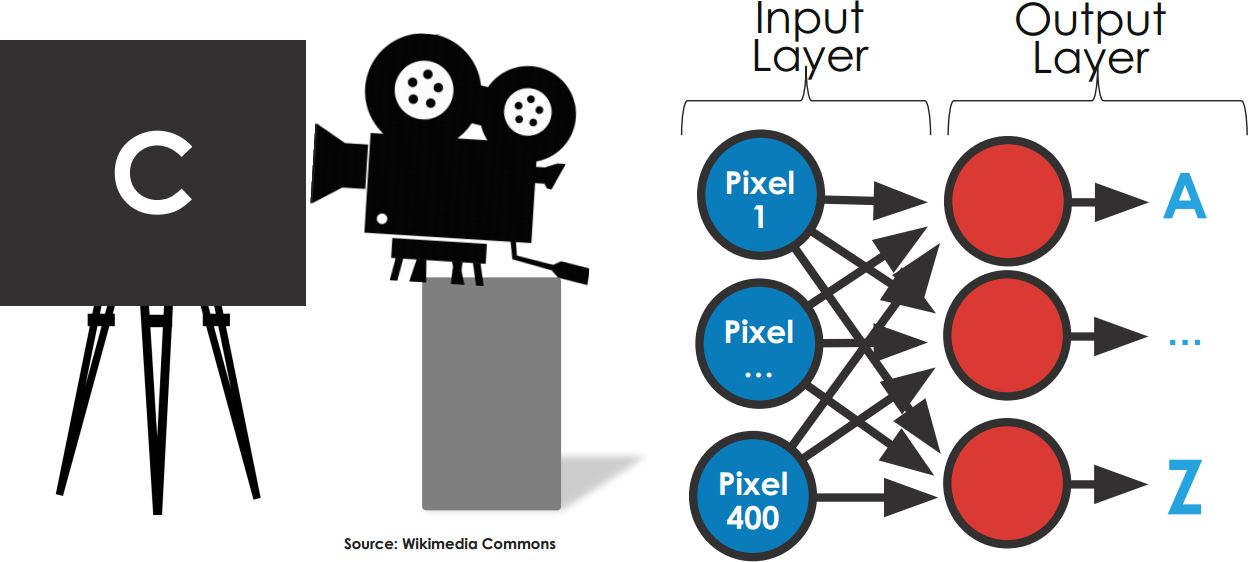
\includegraphics[height=1.3in]{deeplearning1}
		\caption{.}
		\label{fig:deeplearning1}
	\end{figure}

The perceptron assumed a linear relationship which limited its ability (\figurename{}s~\ref{fig:deeplearning2} and~\ref{fig:deeplearning3}).  This started ``AI Winter'' which was a period that artificial intelligence was not funded or researched well.

 	\begin{figure}[tbh]
		\centering
		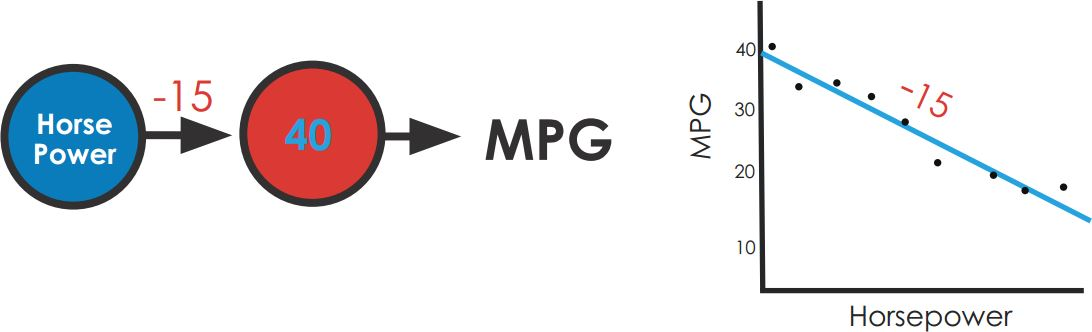
\includegraphics[height=0.9in]{deeplearning2}
		\caption{.}
		\label{fig:deeplearning2}
	\end{figure}

Hidden layers added the ability to model non-linear data (\figurename~\ref{fig:deeplearning4}).  They also added more ``neurons'' in model, either in parallel or serial (\figurename{}s~\ref{fig:deeplearning5} and~\ref{fig:deeplearning6}).  The input neurons are limited to the number of features.

 	\begin{figure}[h]
		\centering
		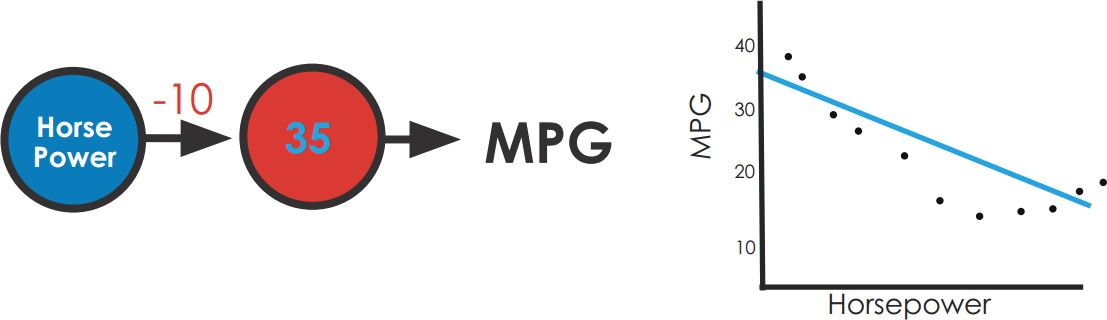
\includegraphics[height=0.9in]{deeplearning3}
		\caption{.}
		\label{fig:deeplearning3}
	\end{figure}

 	\begin{figure}[h]
		\centering
		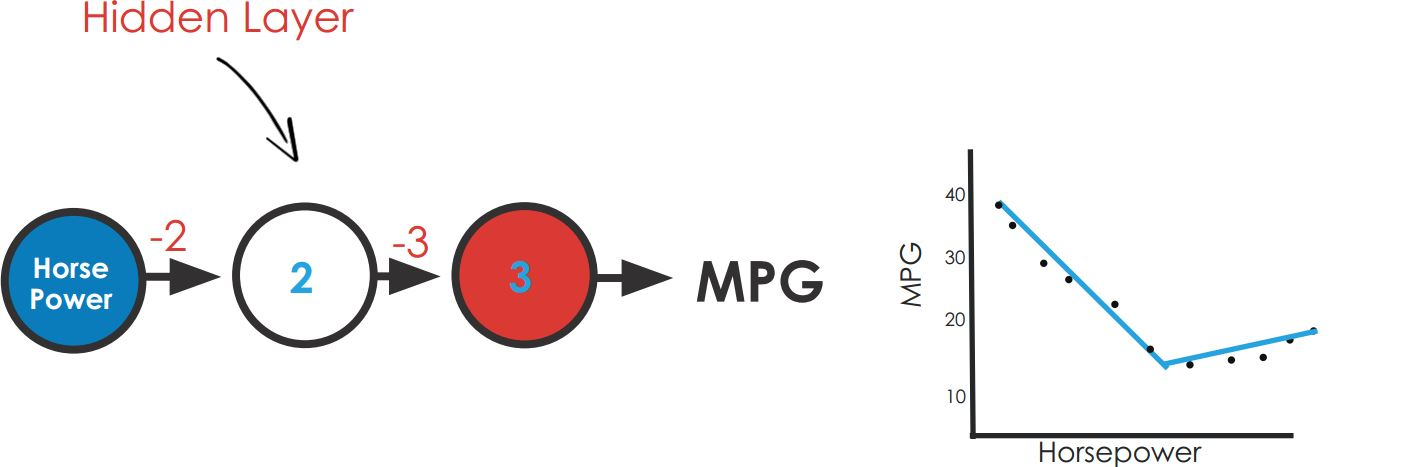
\includegraphics[height=1.0in]{deeplearning4}
		\caption{.}
		\label{fig:deeplearning4}
	\end{figure}

 	\begin{figure}[h]
		\centering
		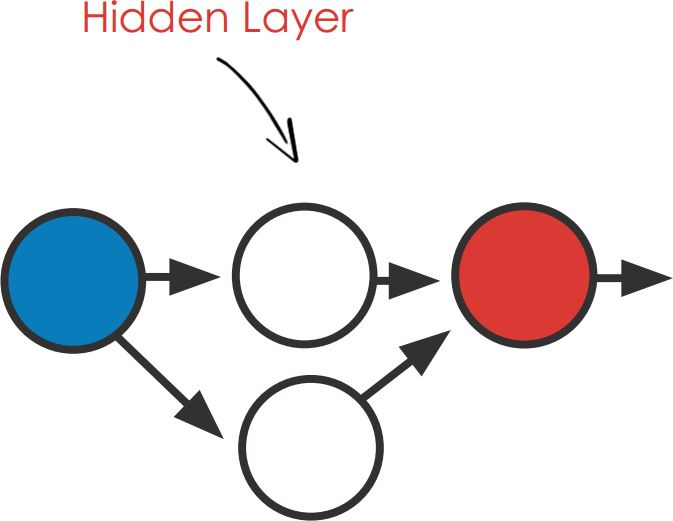
\includegraphics[height=1.1in]{deeplearning5}
		\caption{.}
		\label{fig:deeplearning5}
	\end{figure}

 	\begin{figure}[h]
		\centering
		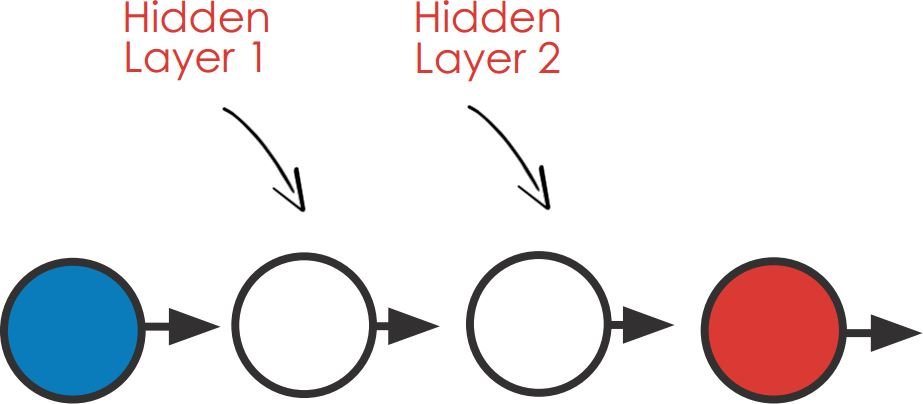
\includegraphics[height=0.9in]{deeplearning6}
		\caption{.}
		\label{fig:deeplearning6}
	\end{figure}

 	\begin{figure}[h]
		\centering
		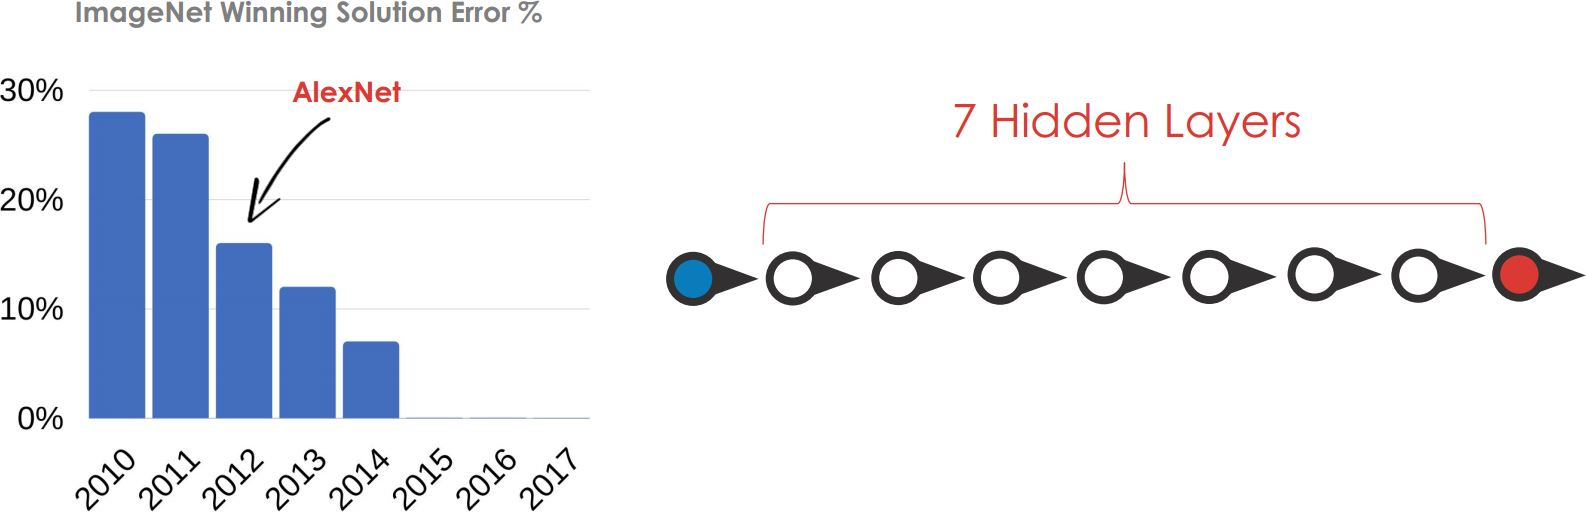
\includegraphics[height=1.5in]{deeplearning7}
		\caption{.}
		\label{fig:deeplearning7}
	\end{figure}

GPT3 was a model with 96 hidden layers trained on text from the internet that could generate articles.

 	\begin{figure}[h]
		\centering
		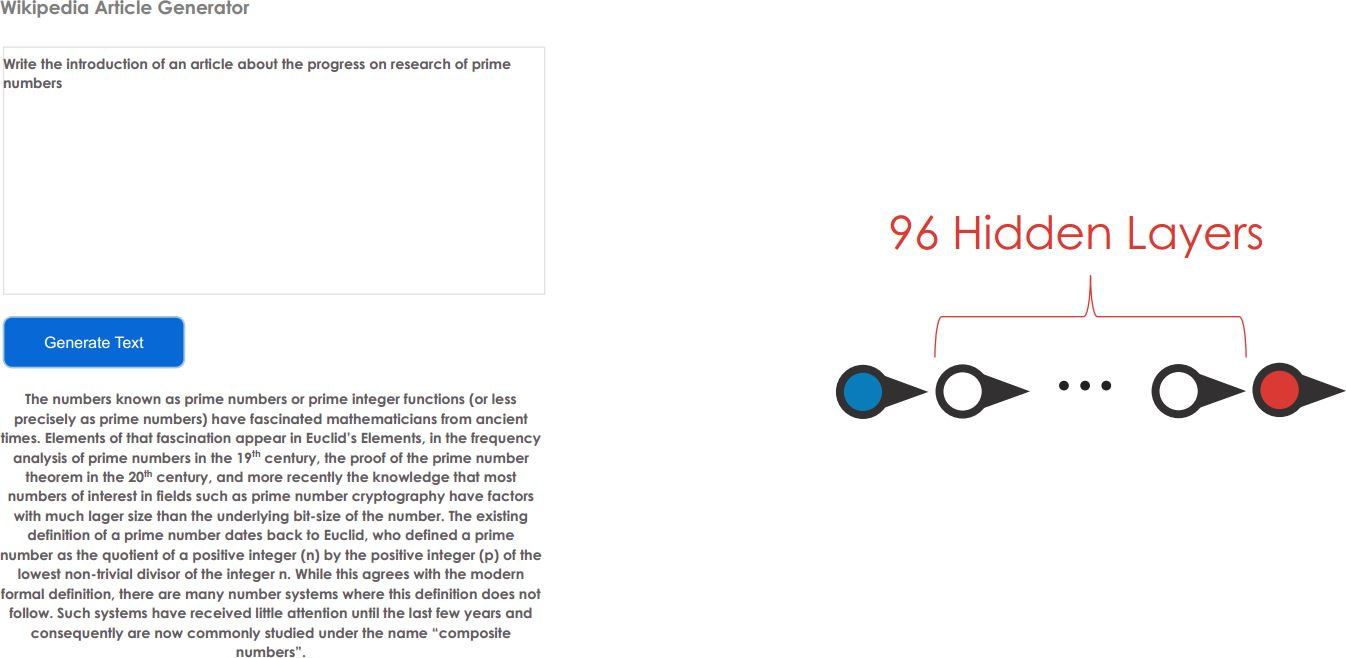
\includegraphics[height=2.2in]{deeplearning8}
		\caption{.}
		\label{fig:deeplearning8}
	\end{figure}


	\subsection{Activation Functions}

 	\begin{figure}[h]
		\centering
		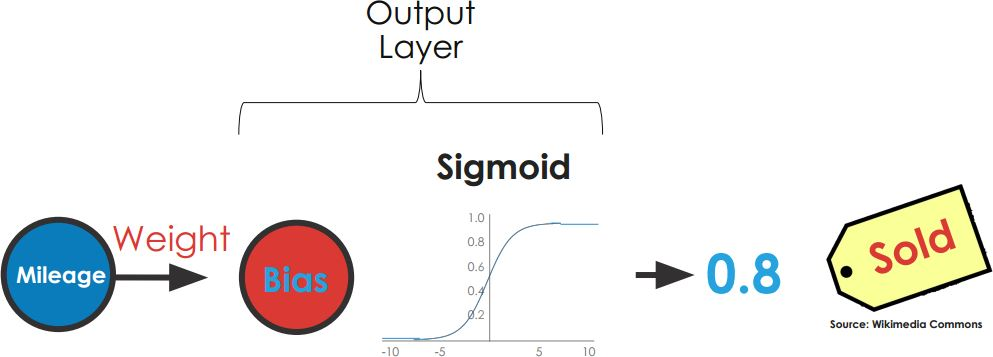
\includegraphics[height=1.1in]{activationfunctionsigmoid}
		\caption{The Sigmoid activation function normalizes the results to be in the range of 0-1.  It is used when the output is binary.}
		\label{fig:activationfunctionsigmoid}
	\end{figure}

 	\begin{figure}[h]
		\centering
		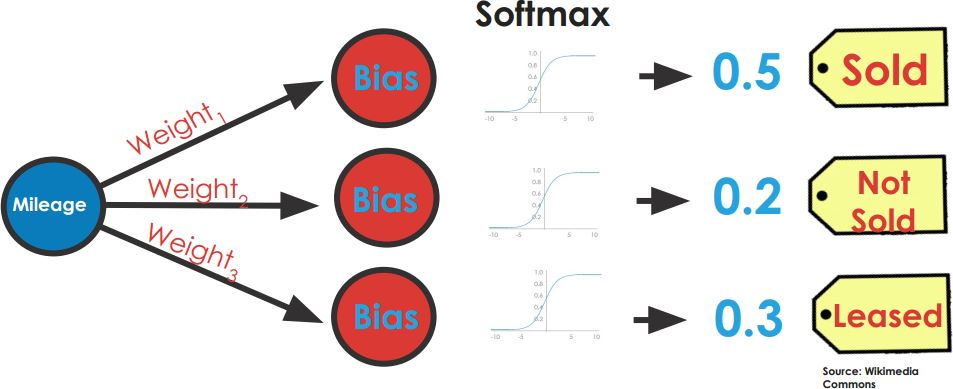
\includegraphics[height=1.1in]{activationfunctionsoftmax}
		\caption{The Softmax activation function normalizes the results to be in the range of 0-1.  It is used when there are multiple classification output categories.}
		\label{fig:activationfunctionsoftmax}
	\end{figure}

 	\begin{figure}[h]
		\centering
		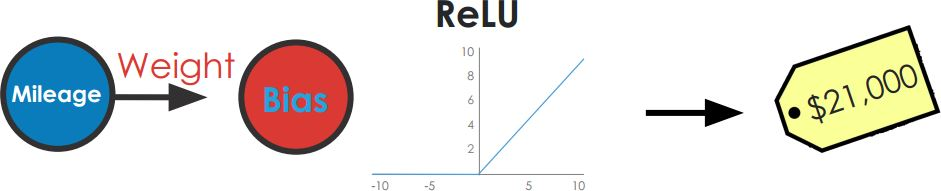
\includegraphics[height=0.85in]{activationfunctionrelu}
		\caption{The ReLu activation function is used for regression.  It prevents negative values (forces to zero).  Positive values are left as is.}
		\label{fig:activationfunctionrelu}
	\end{figure}

Activation functions are used on both the output and hidden layers (see \figurename~\ref{fig:activationfunctionshiddenlayers}).  Without using activation functions on hidden layers, the output is a linear equation.  By adding the activation functions, we can model non-linear functions.

 	\begin{figure}[h]
		\centering
		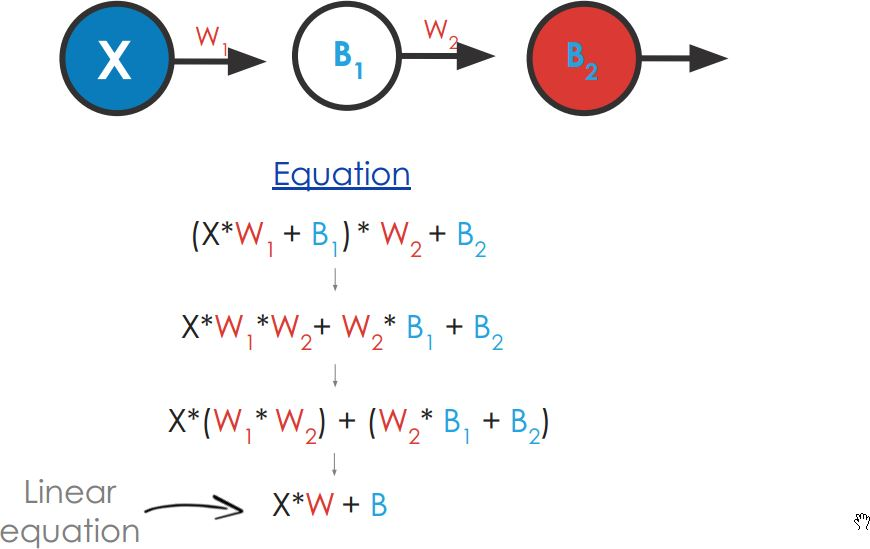
\includegraphics[height=1.5in]{activationfunctionshiddenlayers}
		\caption{Activation functions on hidden layers.}
		\label{fig:activationfunctionshiddenlayers}
	\end{figure}

Sigmoid and Tanh have the problem of a vanishing gradient descent.  The asymptotic nature of the functions means a gradient descent cannot change much in the regions of the small slope.

The Leaky ReLU prevents having all zeros in the negative region.  Having zeros means it kills the path and we loose information.  By having a small negative slope we can retain some of this information.

 	\begin{figure}[h]
		\centering
		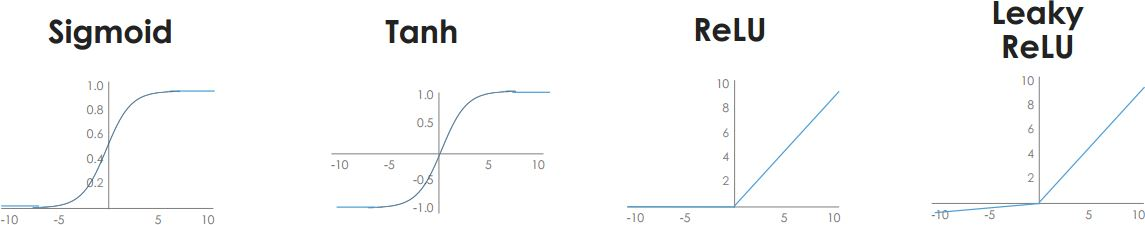
\includegraphics[height=0.85in]{activationfunctiontypes}
		\caption{Popular activation functions.}
		\label{fig:activationfunctiontypes}
	\end{figure}

	\subsection{Gradient Descent}

 	\begin{figure}[h]
		\centering
		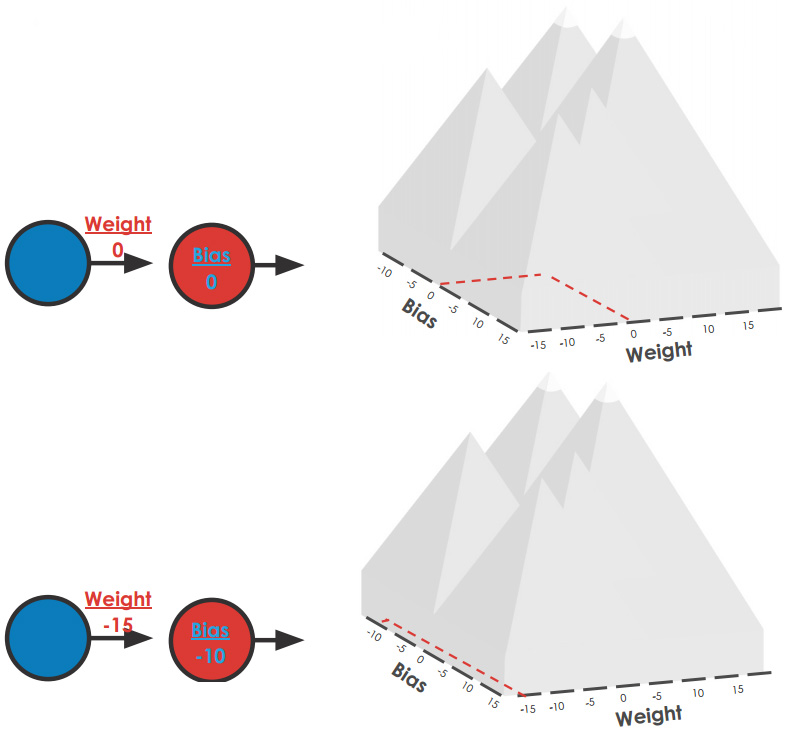
\includegraphics[height=3.0in]{gradientdescent1}
		\caption{}
		\label{fig:gradientdescent1}
	\end{figure}


 	\begin{figure}[h]
		\centering
		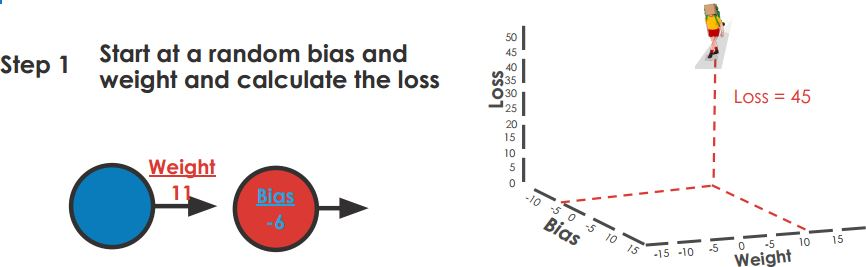
\includegraphics[height=1.5in]{gradientdescentstep1}
		\caption{Gradient descent step 1.}
		\label{fig:gradientdescentstep1}
	\end{figure}

 	\begin{figure}[h]
		\centering
		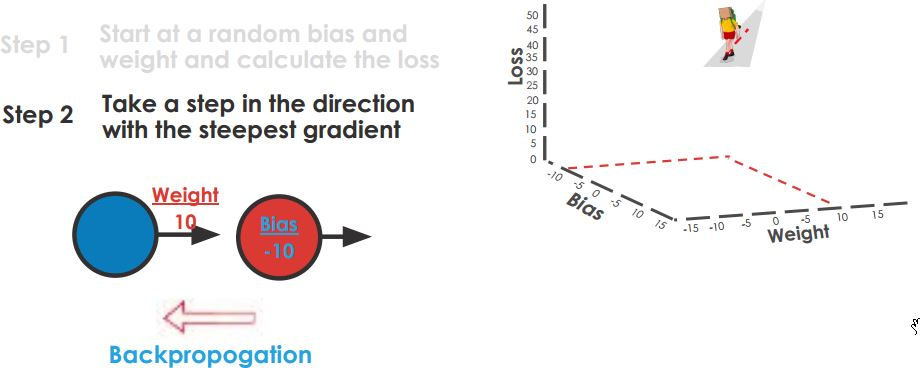
\includegraphics[height=2.0in]{gradientdescentstep2}
		\caption{Gradient descent step 2.}
		\label{fig:gradientdescentstep2}
	\end{figure}

 	\begin{figure}[h]
		\centering
		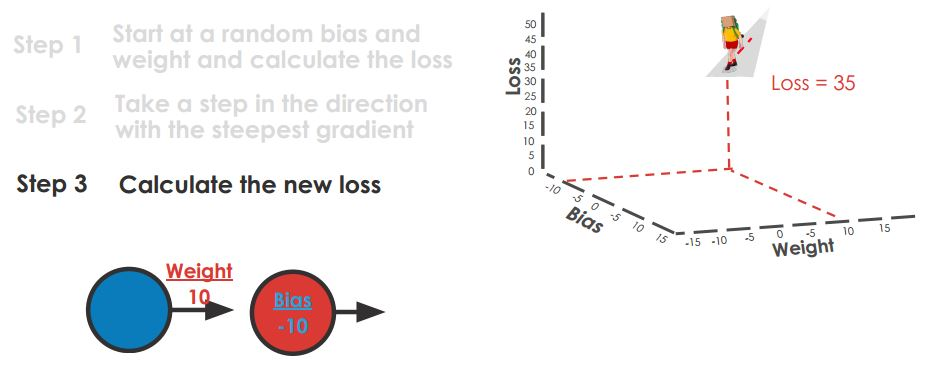
\includegraphics[height=2.0in]{gradientdescentstep3}
		\caption{Gradient descent step 3.}
		\label{fig:gradientdescentstep3}
	\end{figure}

 	\begin{figure}[h]
		\centering
		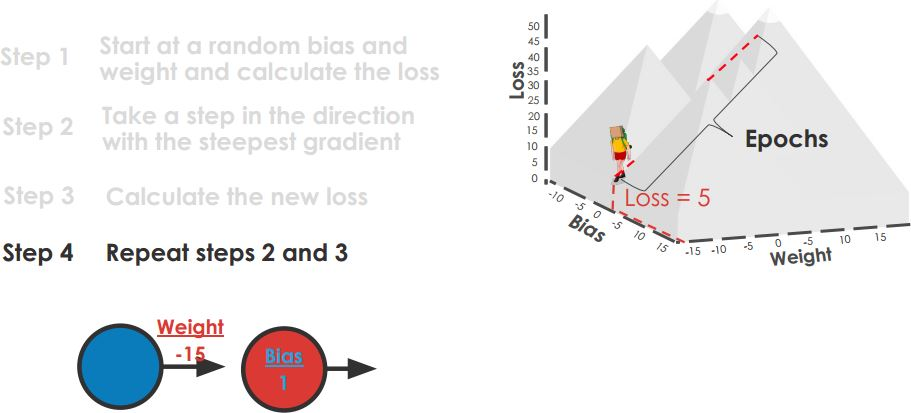
\includegraphics[height=2.0in]{gradientdescentstep4}
		\caption{Gradient descent step 4.}
		\label{fig:gradientdescentstep4}
	\end{figure}

	\subsubsection{Calculating the Descent}

 	\begin{figure}[h]
		\centering
		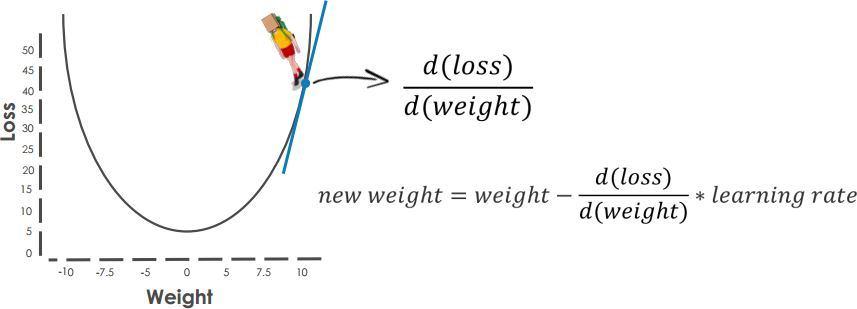
\includegraphics[height=1.5in]{gradientdescentcalculatingthegradient1}
		\caption{}
		\label{fig:gradientdescentcalculatingthegradient1}
	\end{figure}

 	\begin{figure}[h]
		\centering
		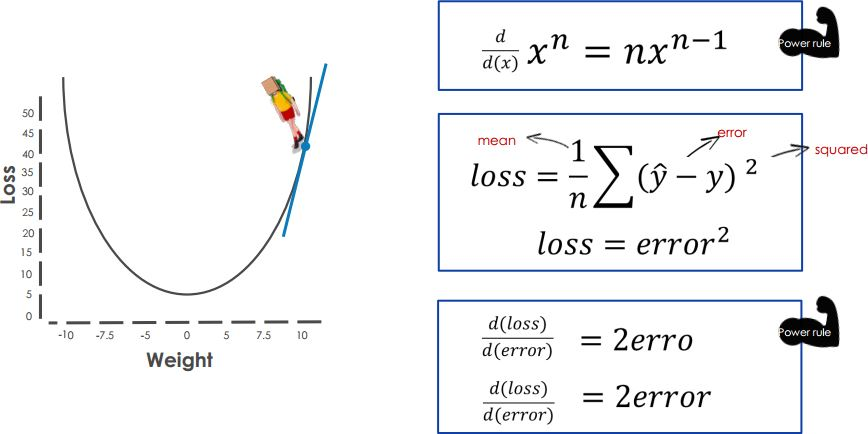
\includegraphics[height=1.5in]{gradientdescentcalculatingthegradient2}
		\caption{}
		\label{fig:gradientdescentcalculatingthegradient2}
	\end{figure}

 	\begin{figure}[h]
		\centering
		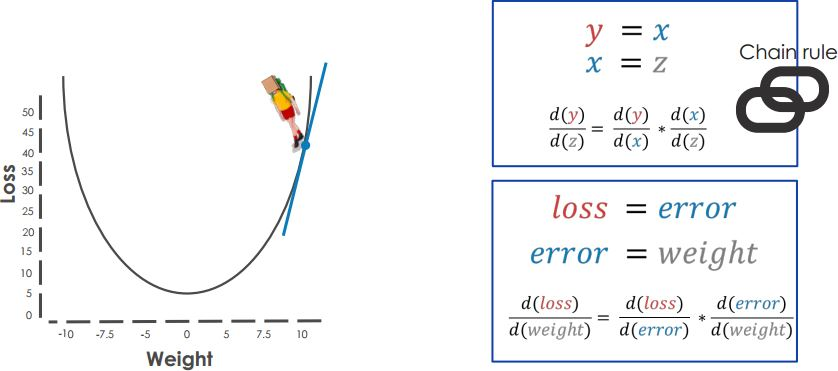
\includegraphics[height=1.5in]{gradientdescentcalculatingthegradient3}
		\caption{}
		\label{fig:gradientdescentcalculatingthegradient3}
	\end{figure}

 	\begin{figure}[h]
		\centering
		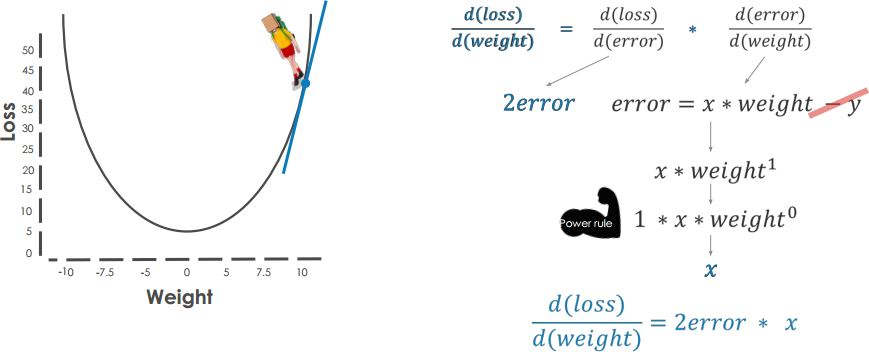
\includegraphics[height=1.5in]{gradientdescentcalculatingthegradient4}
		\caption{}
		\label{fig:gradientdescentcalculatingthegradient4}
	\end{figure}

 	\begin{figure}[h]
		\centering
		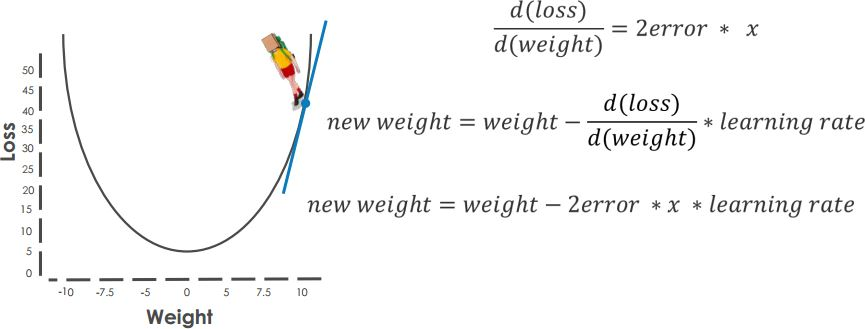
\includegraphics[height=1.5in]{gradientdescentcalculatingthegradient5}
		\caption{}
		\label{fig:gradientdescentcalculatingthegradient5}
	\end{figure}

	\subsection{Gradient Descent Optimization Parameters}
The parameters used for tuning the gradient decent algorithm are shown in \tablename~\ref{tab:gradientdescentoptimization}.

    \begin{topcaptiontable}
        \centering
        \lecaption{Comparison of hyperparameters used to tune the performance of the gradient descent algorithm.}
        \label{tab:gradientdescentoptimization}
		\begin{tabular}{|l|p{0.8\textwidth}|} \hline
				\tablecolumnheadervlinesone{Parameter} & \tablecolumnheadervlinestwo{Description} \\ \hline
				epochs &
	            The number of times the data is fed through the gradient descent process.  It is possible to over fit the data if too many epochs are used. \\ \hline
				batch size &
				The amount of the data used to calculate the gradient.  Batch is to use all the data.  Mini-batch is to use a subset of the data.  Stochastic is to use one sample of the data. \\ \hline
				learning rate &
				The step size used to update the values. \\ \hline
				optimizers &
				Momentum optimizer takes into account the direction you were heading to continue over small hills and prevent getting stuck on local minimums.  Adagrad helps avoid over shooting the global minimum by slowing down the learning rate on long slops.  RMSprop can slow or speed up learning rate.  The Adam optimizer combines the elements of all the other optimizers. \\ \hline
				steps &
				The steps are not directly controllable, rather they are the function of the batch size ($s_b$), data size ($s_d$), and number of epochs ($n_e$), i.e. $\frac{s_d}{s_b}*n_e$ \\ \hline
		\end{tabular}
	\end{topcaptiontable}

The epochs and batch size are closely related.  The larger the batch size the fewer the number of


 	\begin{figure}[h]
		\centering
		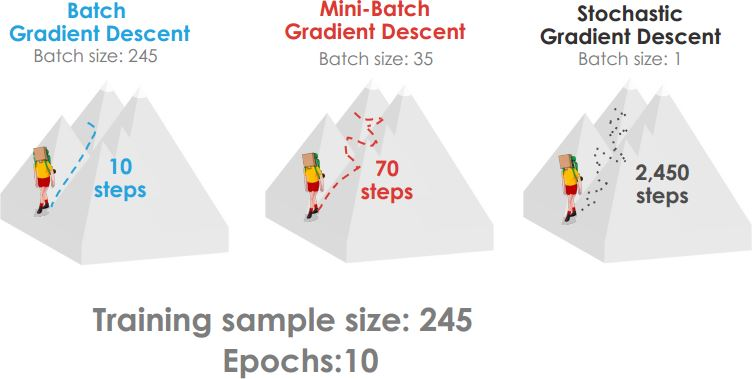
\includegraphics[height=1.5in]{gradientdescentoptimization1}
		\caption{}
		\label{fig:gradientdescentoptimization1}
	\end{figure}

	\begin{equation}
		\textrm{new} = \textrm{old} - \textrm{gradient} * \textrm{learning\_rate}
	\end{equation}



	\subsection{Normalizing}

 	\begin{figure}[h]
		\centering
		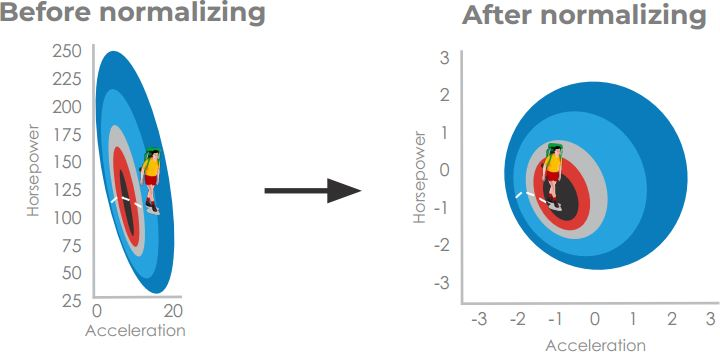
\includegraphics[height=1.5in]{normalizing}
		\caption{}
		\label{fig:normalizing}
	\end{figure}

	\section{Artificial Neural Network Hyperparameter Tuning}

 	\begin{figure}[h]
		\centering
		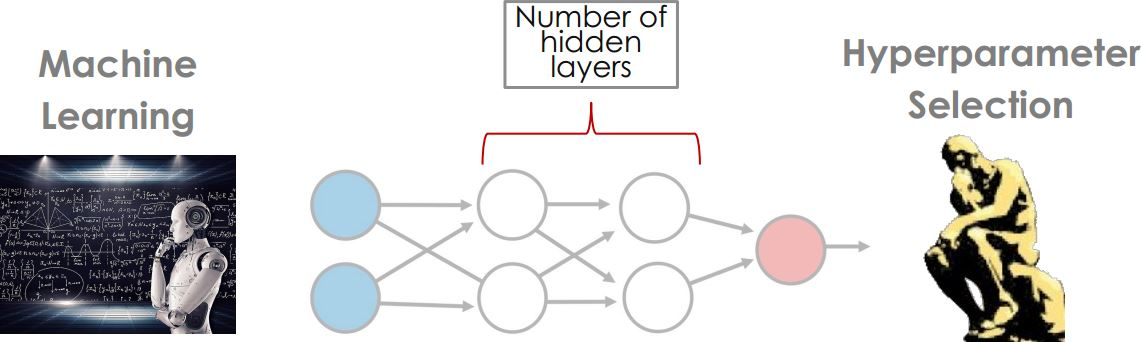
\includegraphics[height=1.2in]{artificialneuralnetworkshyperparameter1}
		\caption{}
		\label{fig:artificialneuralnetworkshyperparameter1}
	\end{figure}
 	\begin{figure}[h]
		\centering
		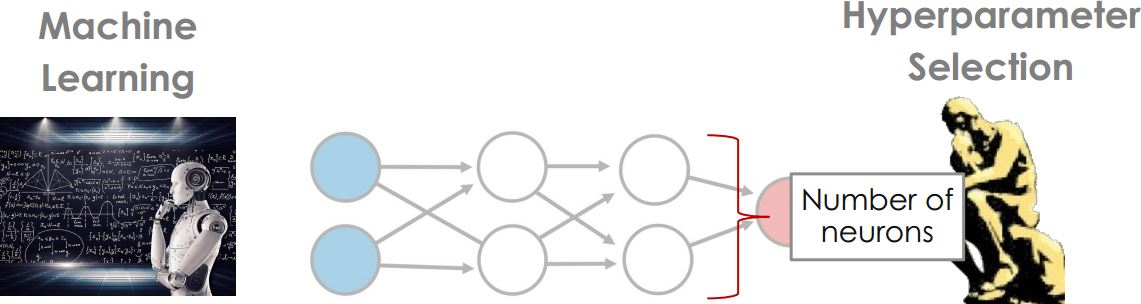
\includegraphics[height=1.2in]{artificialneuralnetworkshyperparameter2}
		\caption{}
		\label{fig:artificialneuralnetworkshyperparameter2}
	\end{figure}
 	\begin{figure}[h]
		\centering
		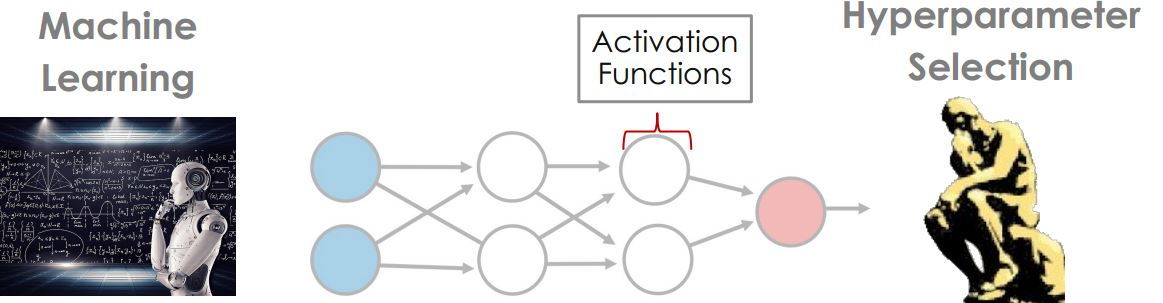
\includegraphics[height=1.2in]{artificialneuralnetworkshyperparameter3}
		\caption{}
		\label{fig:artificialneuralnetworkshyperparameter3}
	\end{figure}
 	\begin{figure}[h]
		\centering
		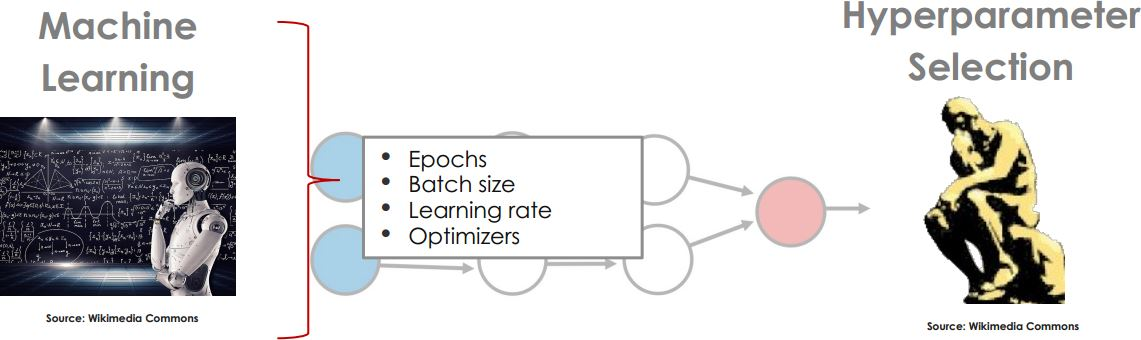
\includegraphics[height=1.2in]{artificialneuralnetworkshyperparameter4}
		\caption{}
		\label{fig:artificialneuralnetworkshyperparameter4}
	\end{figure}
 	\begin{figure}[h]
		\centering
		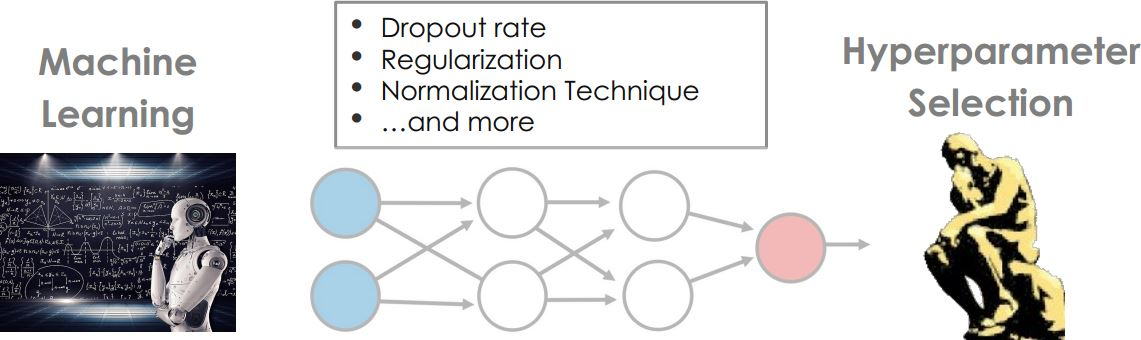
\includegraphics[height=1.2in]{artificialneuralnetworkshyperparameter5}
		\caption{}
		\label{fig:artificialneuralnetworkshyperparameter5}
	\end{figure}
 	\begin{figure}[h]
		\centering
		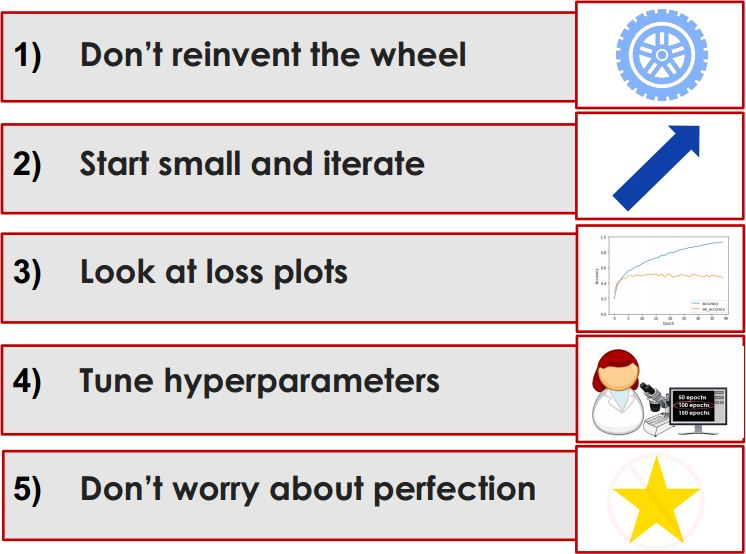
\includegraphics[height=1.2in]{artificialneuralnetworkshyperparameter6}
		\caption{}
		\label{fig:artificialneuralnetworkshyperparameter6}
	\end{figure} 